\chapter{Analysis and Design}
\section{Introduction}
\par
This chapters covers three topics which are user requirement, business process designs, and system design. The user requirement part discusses the business needs for what users require from the system, The business process design part discusses the activities diagram, use case diagram, and context diagram of the application. Lastly, the system design consists of database design, and system architecture.

\section{User definition}
\begin{itemize}
    \item People who aged around 12 - 40 years old and familiar with English language
    \item Lived in Bangkok and in the city crowded with technology-accessible people
    \item People who trying to travel into newly visited place without known directions
    \item People who want to browse alternative transportation method to reach their destination with their own condition like cost savings, faster route, or less transfer
\end{itemize}
\subsection{User persona}
\begin{figure}[!h]
    \centering
    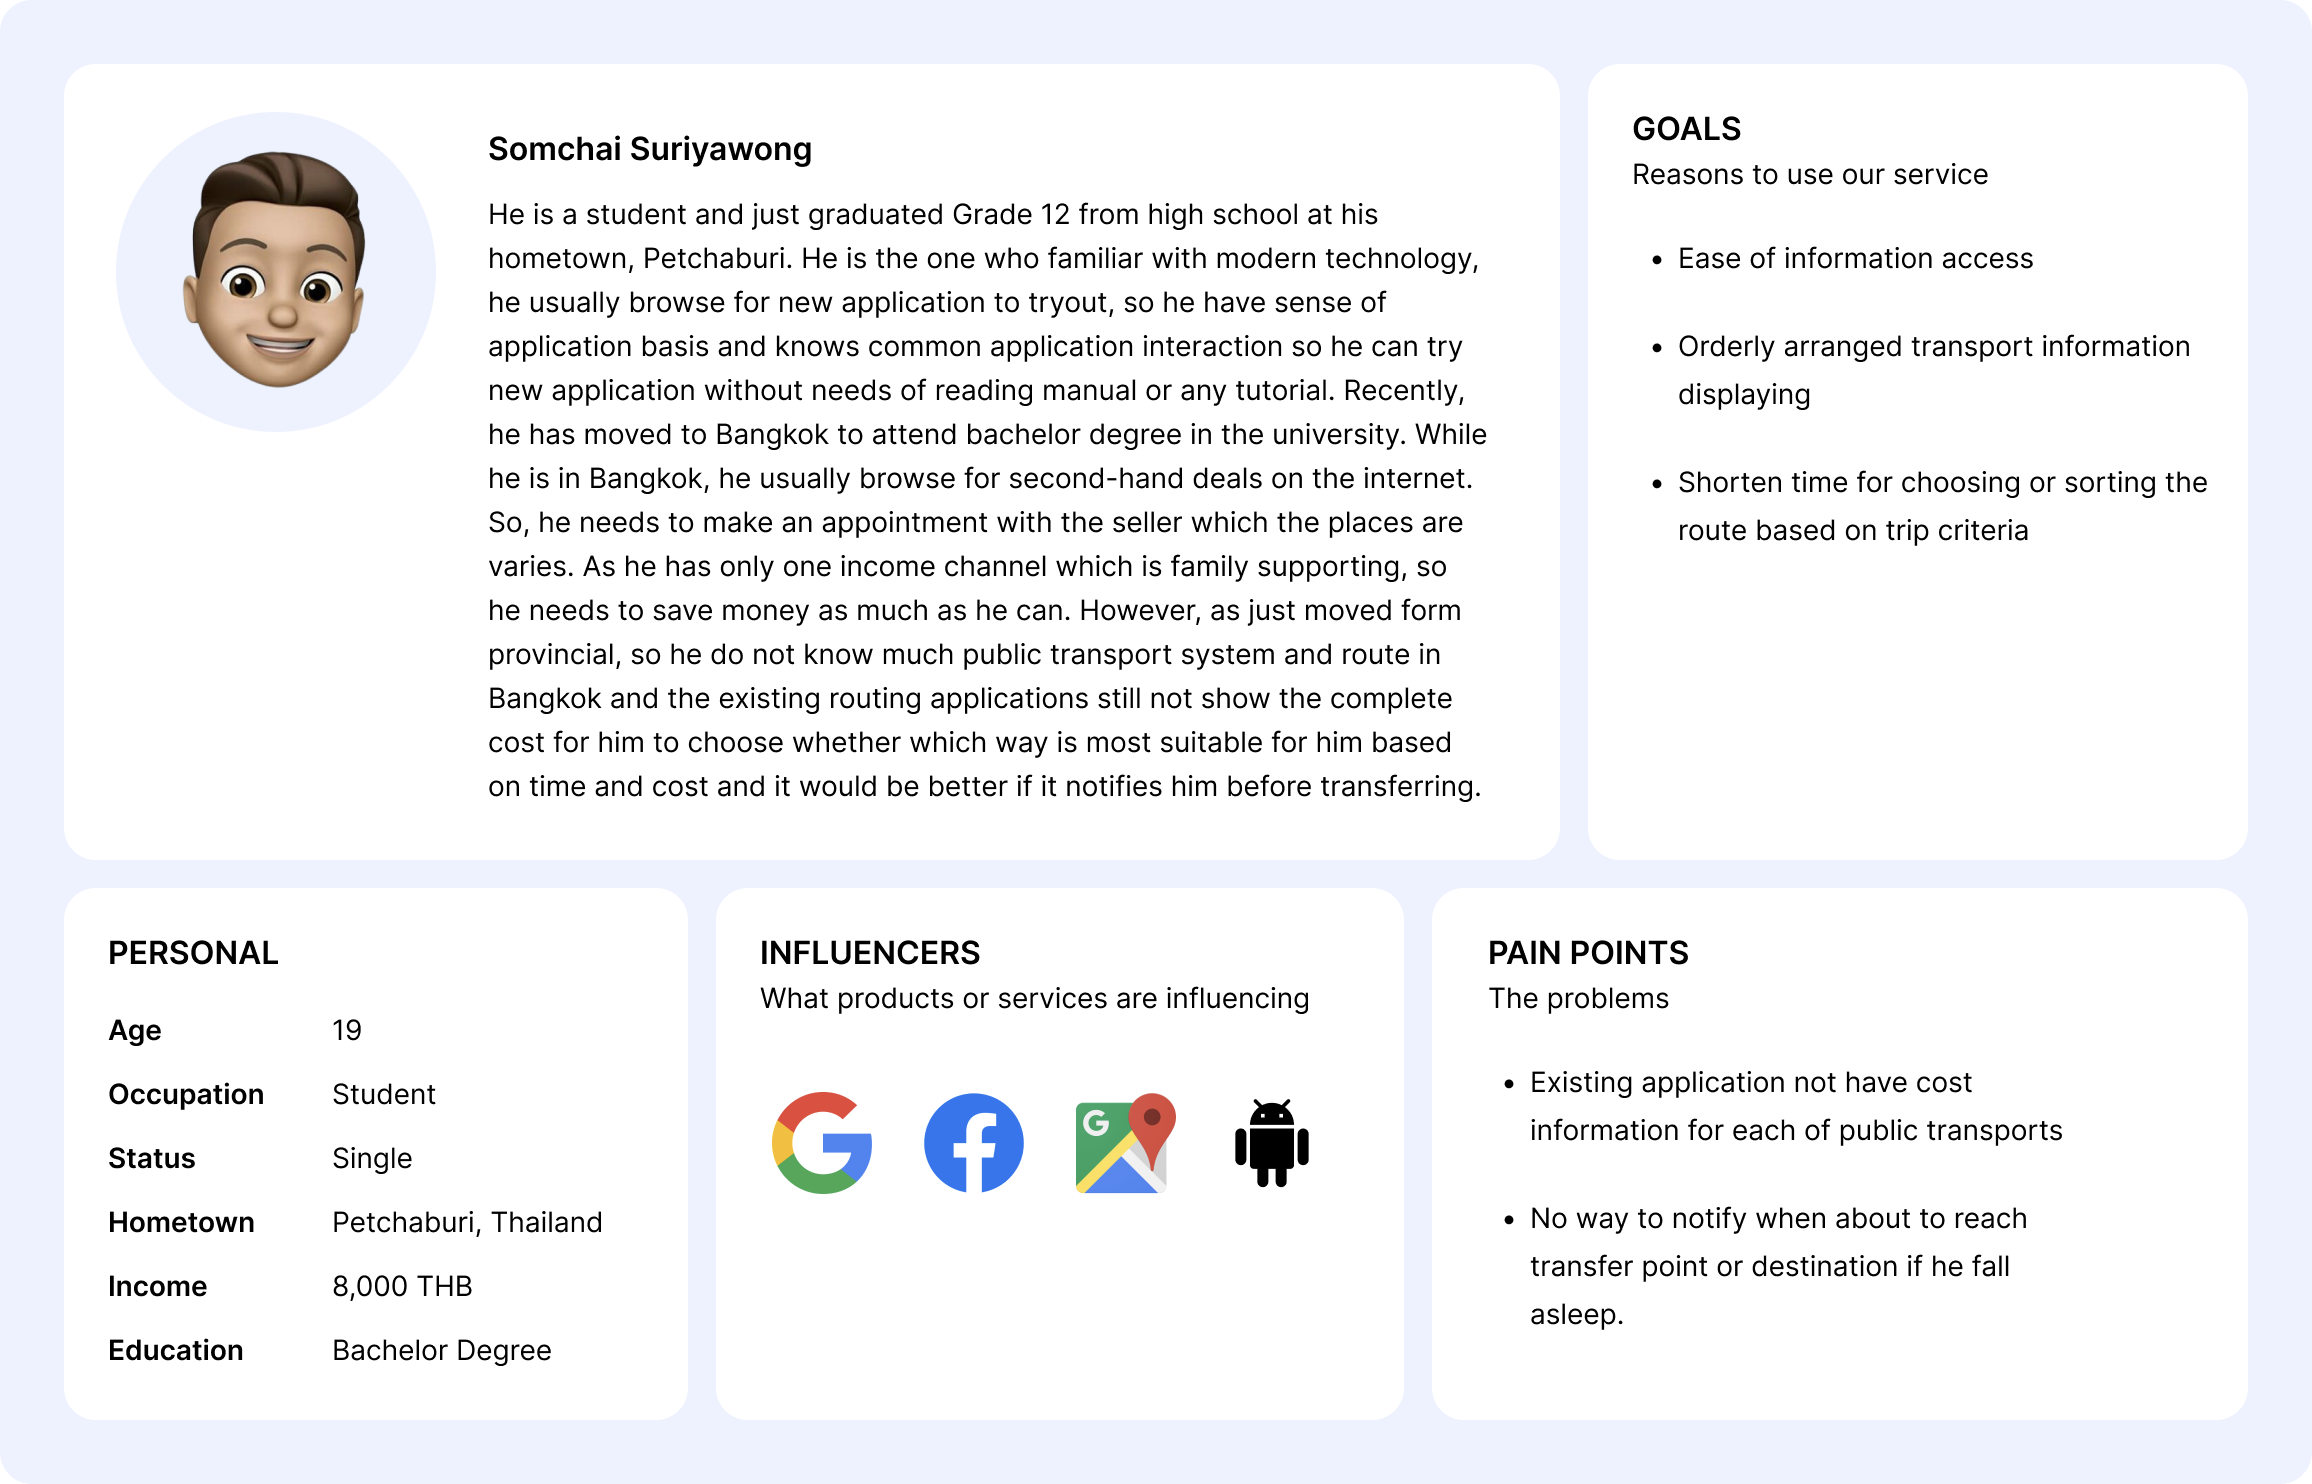
\includegraphics[width=1\linewidth]{chapter3/user-persona-1.png}
    \caption{User one persona}    
    \label{fig:User one persona}
\end{figure}
\begin{figure}[!h]
    \centering
    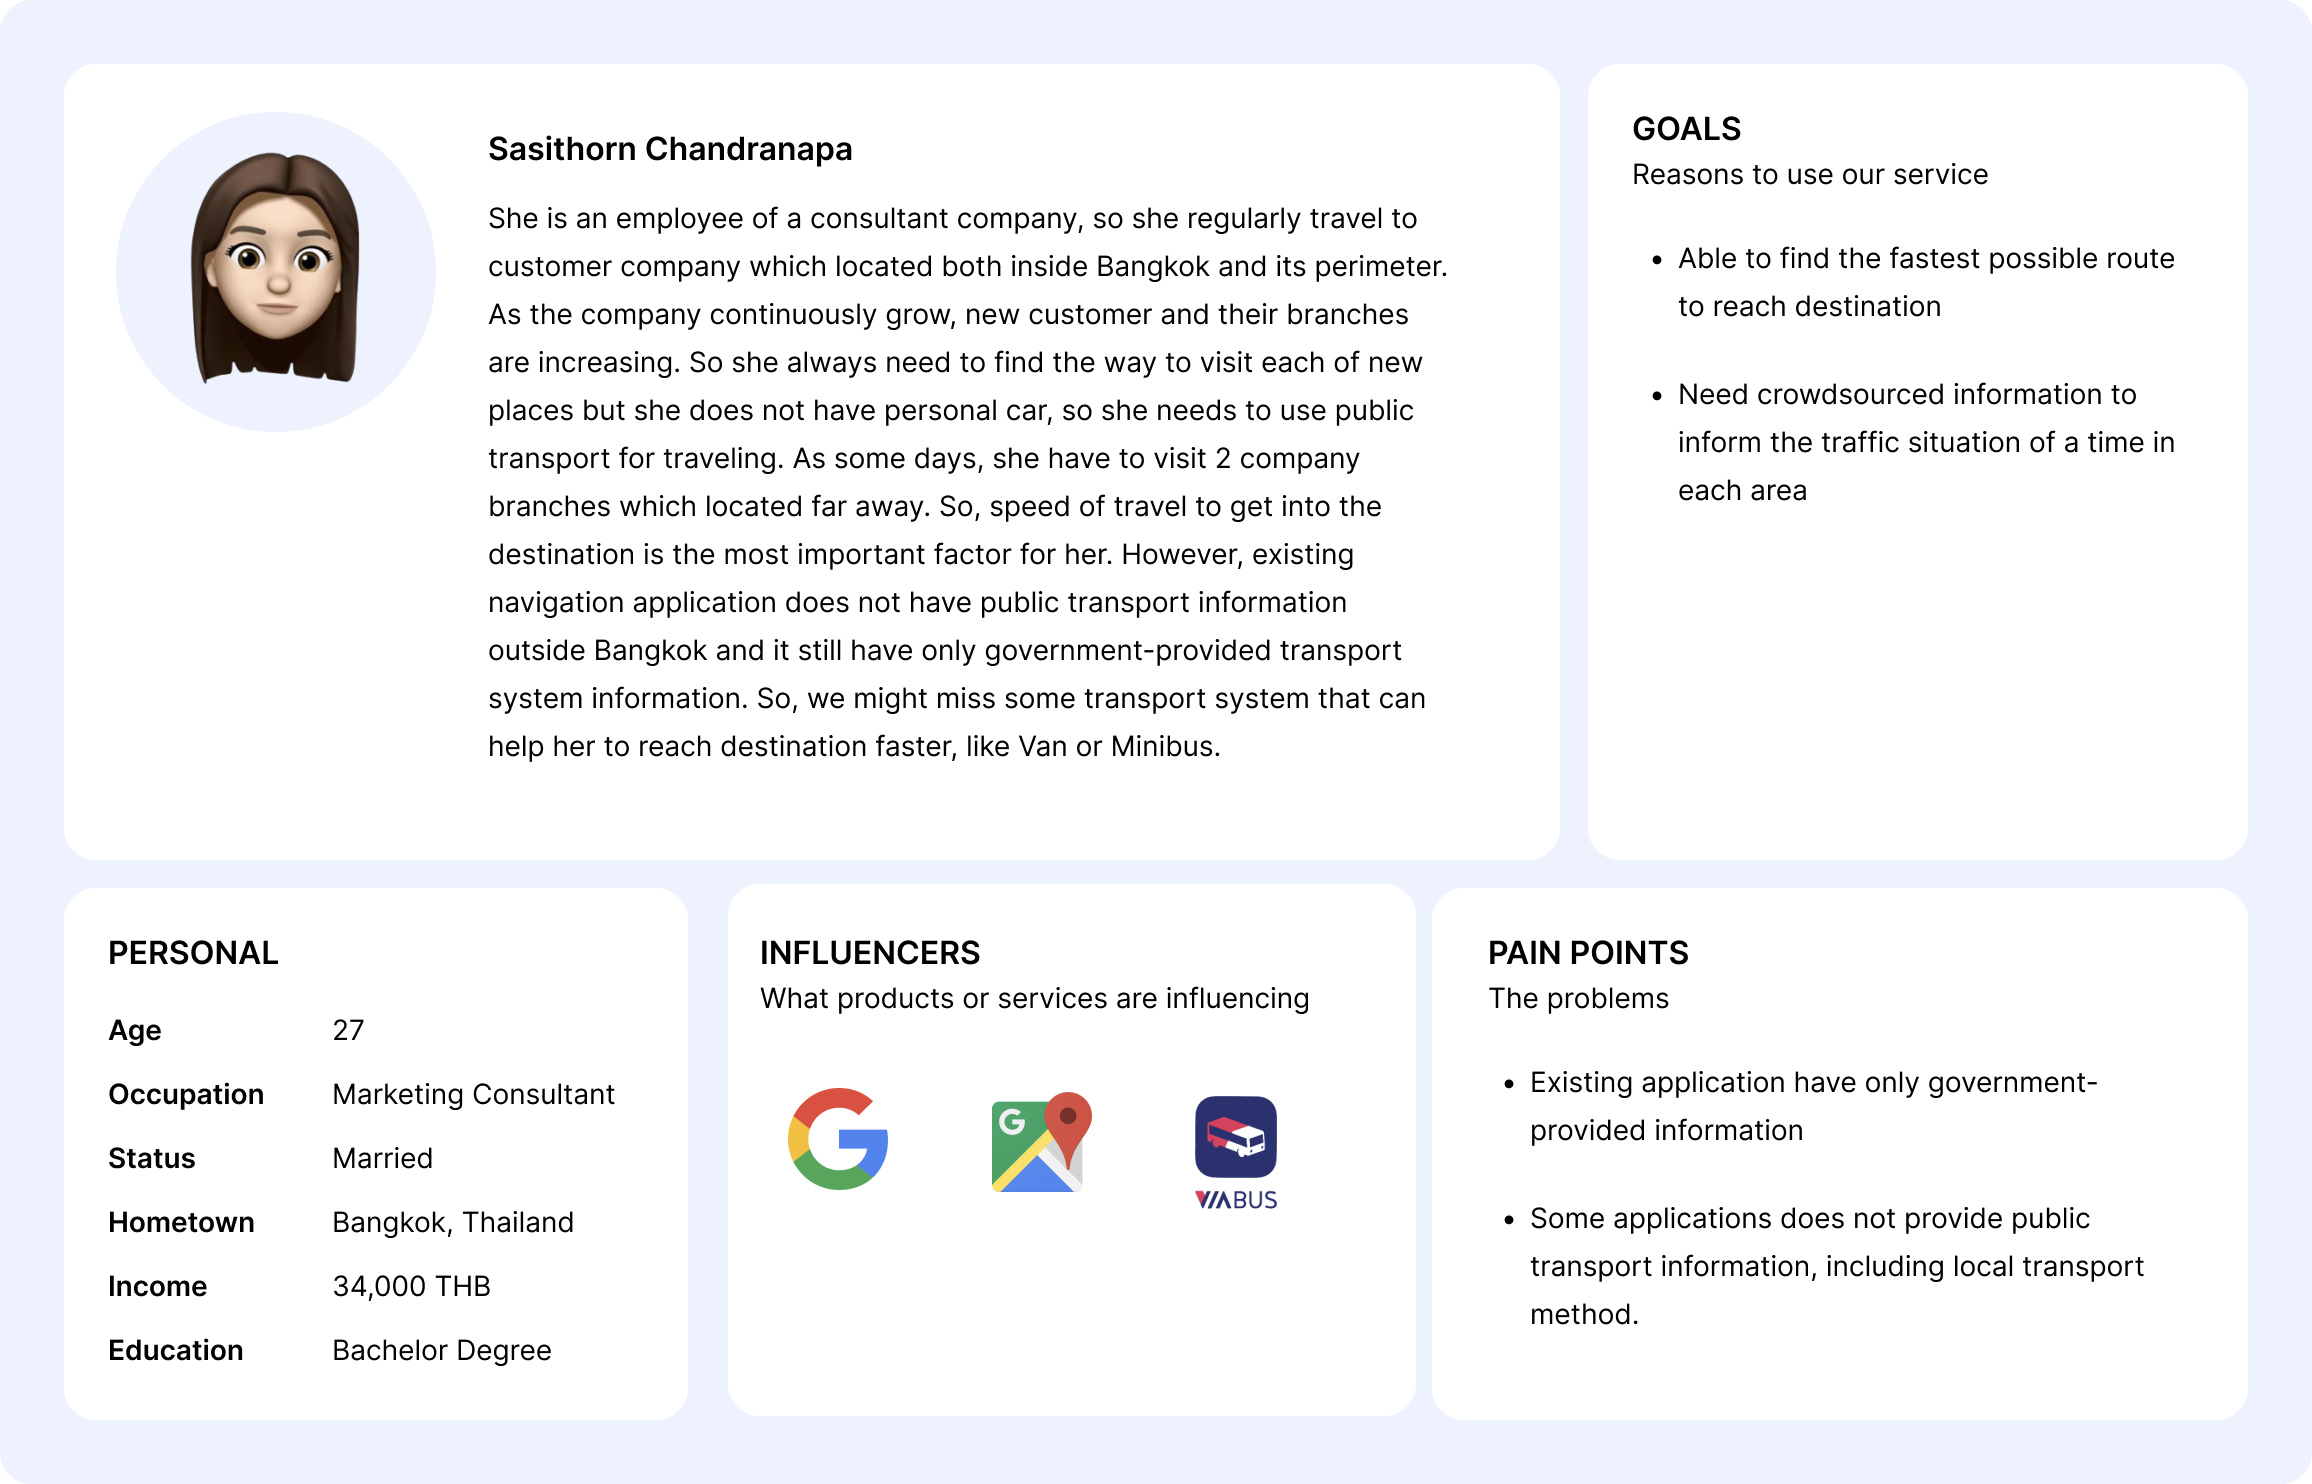
\includegraphics[width=1\linewidth]{chapter3/user-persona-2.png}
    \caption{User two persona}
    \label{fig:User two persona}
\end{figure}
\begin{figure}[!h]
    \centering
    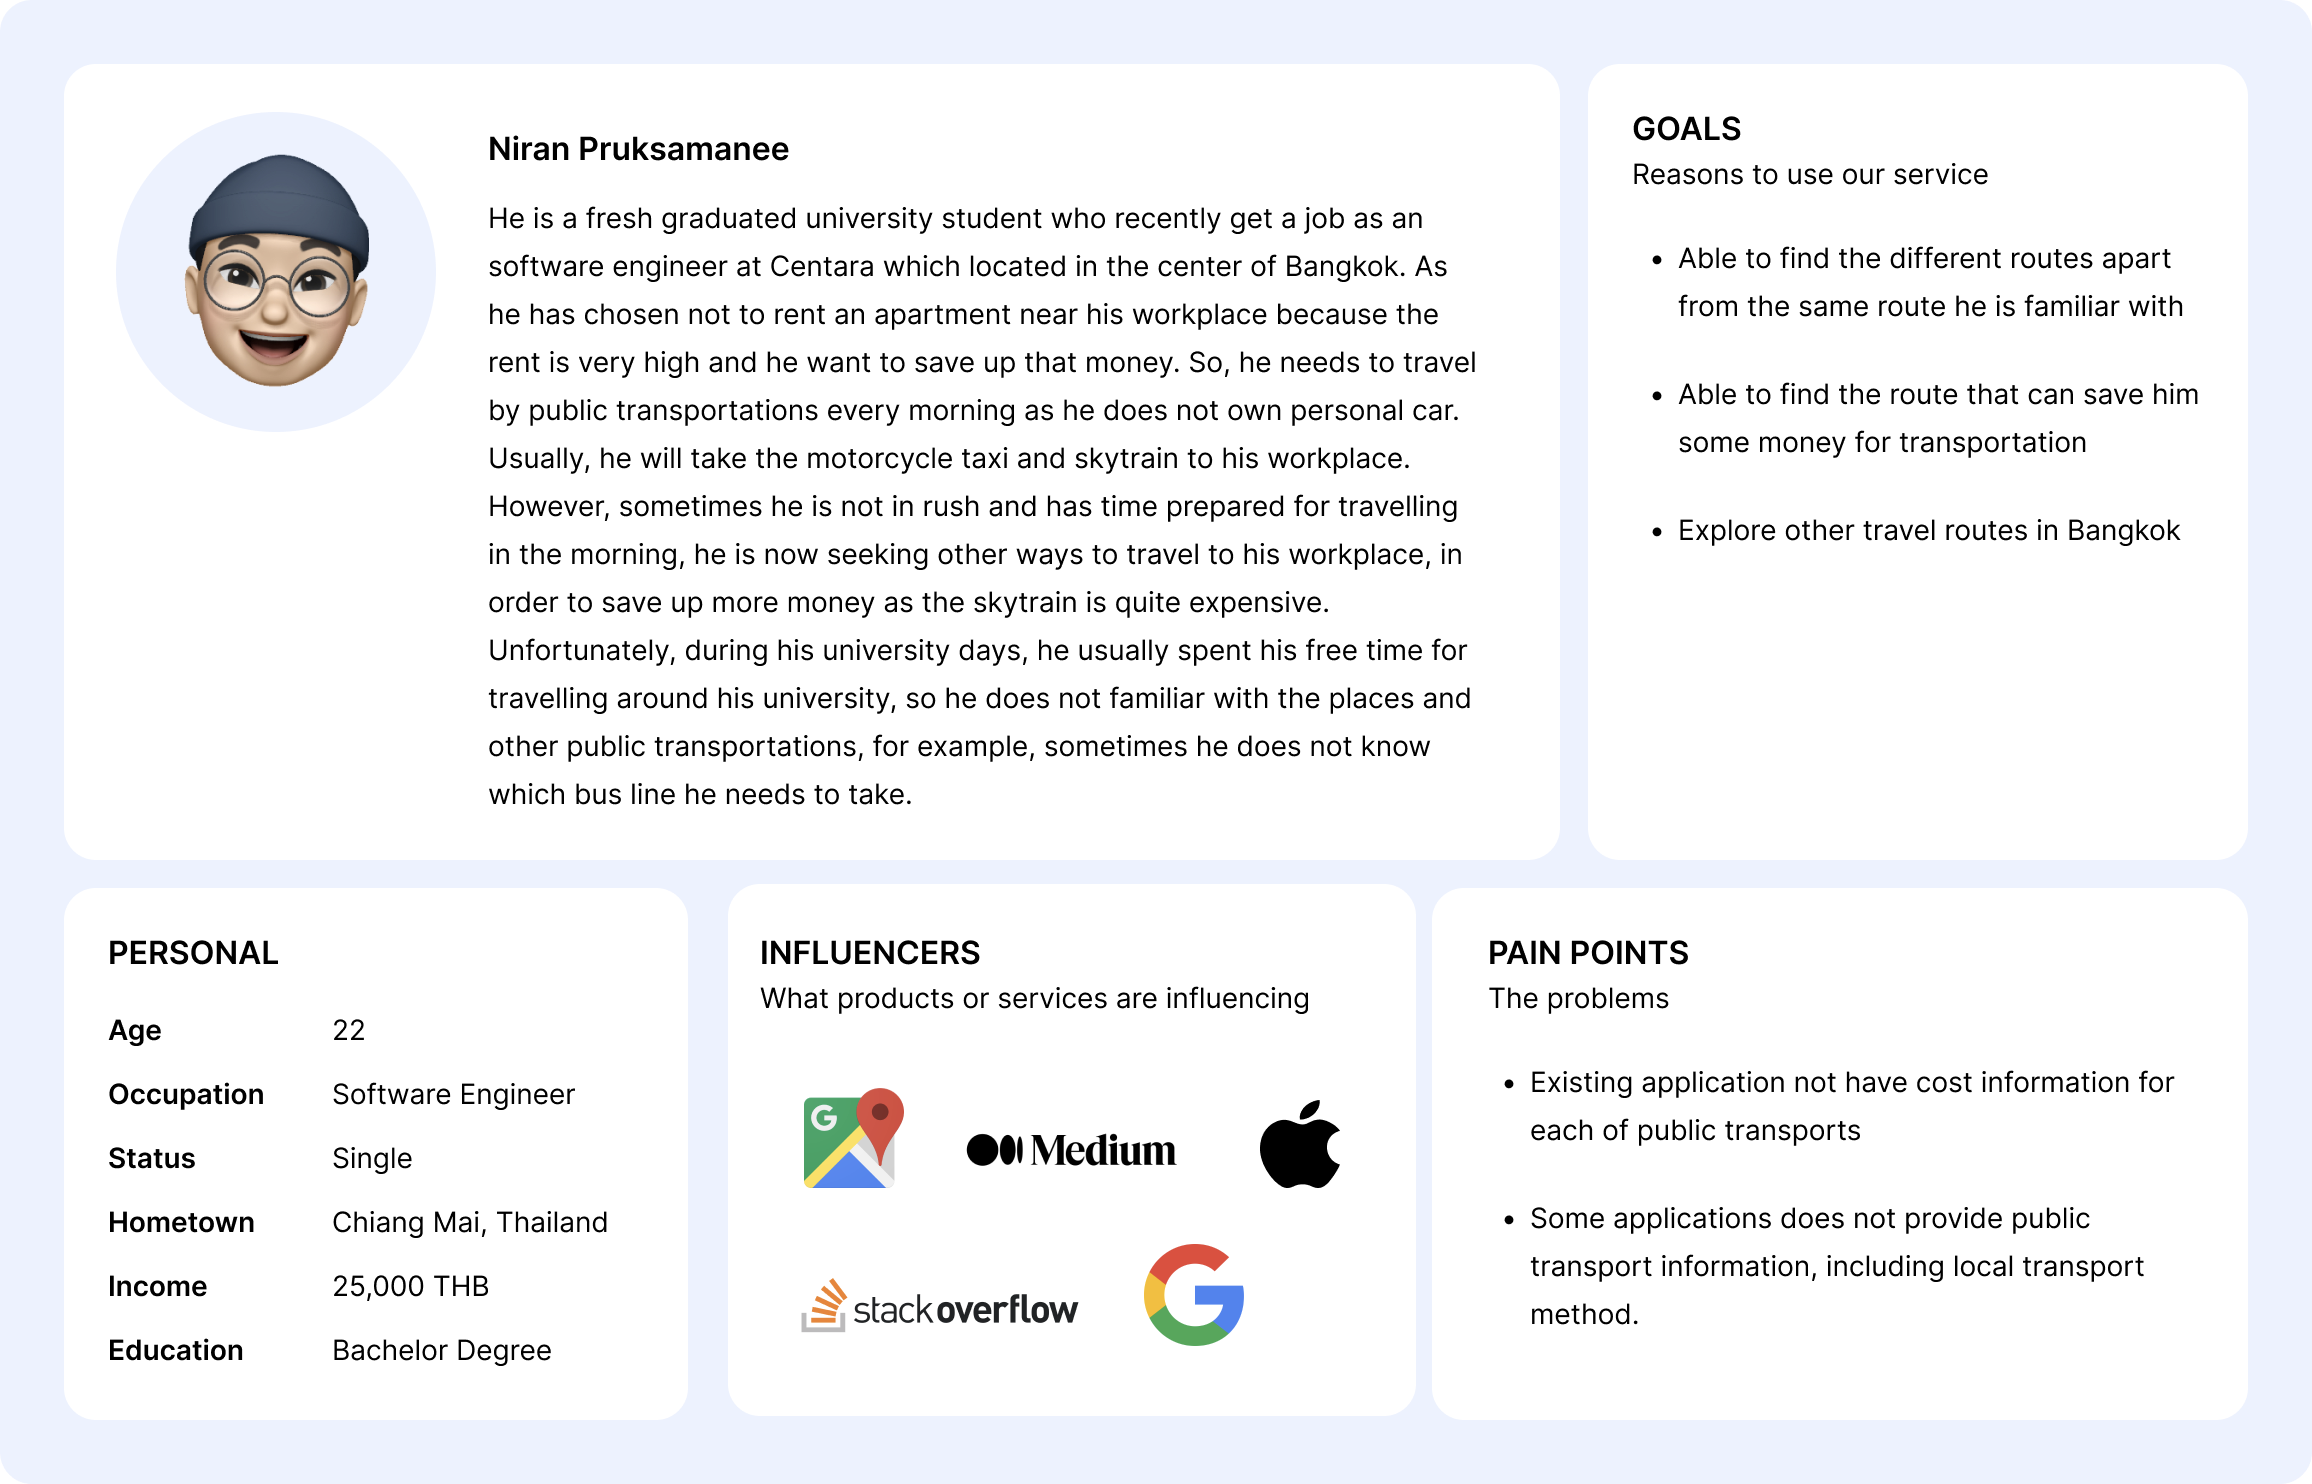
\includegraphics[width=1\linewidth]{chapter3/user-persona-3.png}
    \caption{User three persona}
    \label{fig:User three persona}
\end{figure}
\subsection{User requirement analysis}
\begin{itemize}
    \item This application helps users to find the best route for traveling.
    \item This application uses map service provider and our public transportation data such as vans, and mini truck to suggest the route for users.
    \item This application provides the community to share the routes of traveling of users.
    \item This application will provide a mobile application for users that use smartphones.
\end{itemize}

\section{Use case diagram}
\begin{figure}[!h]
    \centering
    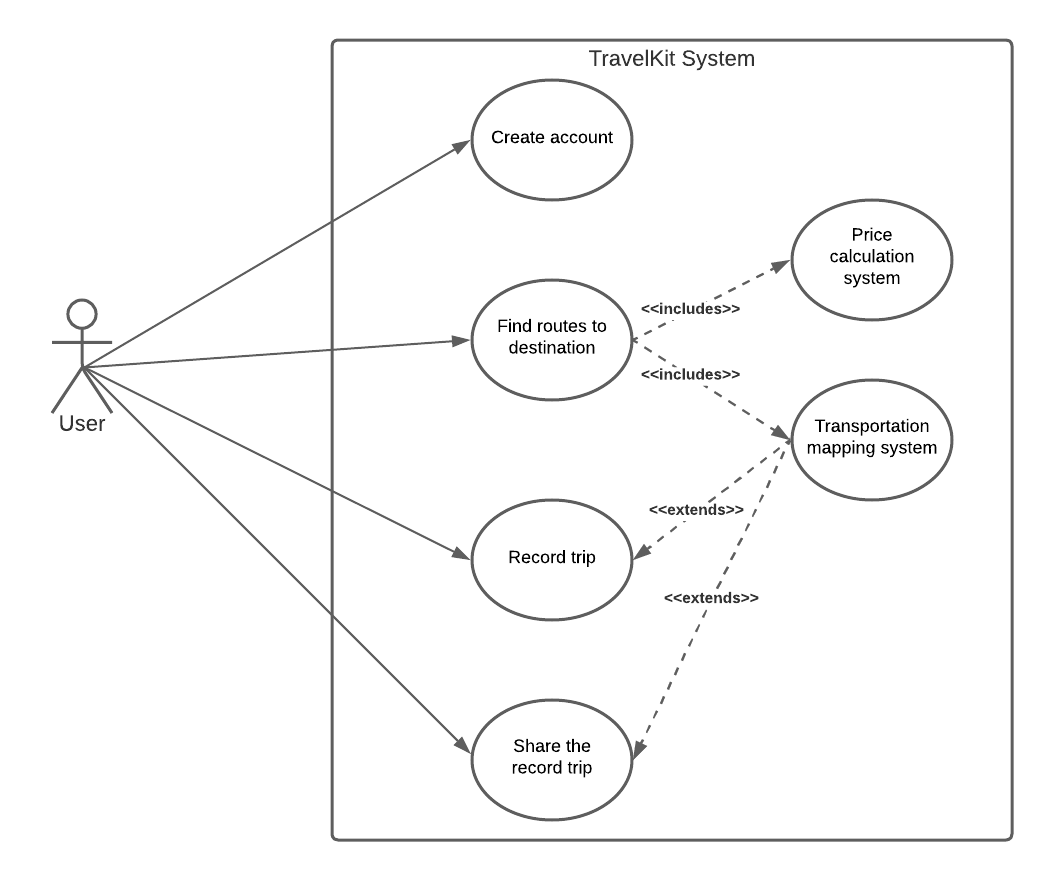
\includegraphics[width=0.7\linewidth]{chapter3/use-case-diagram.png}
    \caption{Use case diagram}
    \label{fig:Use case diagram}
\end{figure}
\par
The actor who is user in the routing system. The user must create an account to login to the system. After the user finds routes to the destination, the system will calculate the cost of traveling and display alternative routes using public transport data, such as vans and mini trucks, so that the user can make informed decisions. In addition, the user can record their trip after reaching the destination. Lastly, the user can share their trip to the community, along with the details of their travel, as well as comment and recommend other users.

\newpage
\section{Context diagram}
\begin{figure}[!h]
    \centering
    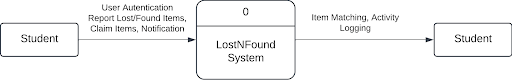
\includegraphics[width=1\linewidth]{chapter3/context-diagram.png}
    \caption{Context diagram}
    \label{fig:Context diagram}
\end{figure}
\par
The context diagram shows the overall of the TravelKit system that required the name, password, user’s location, destination. Then, the system will create choices of the routes, directions and calculate the cost of traveling to the destination.

\section{Activity diagram}
\subsection{Travel process}
\begin{figure}[!h]
    \centering
    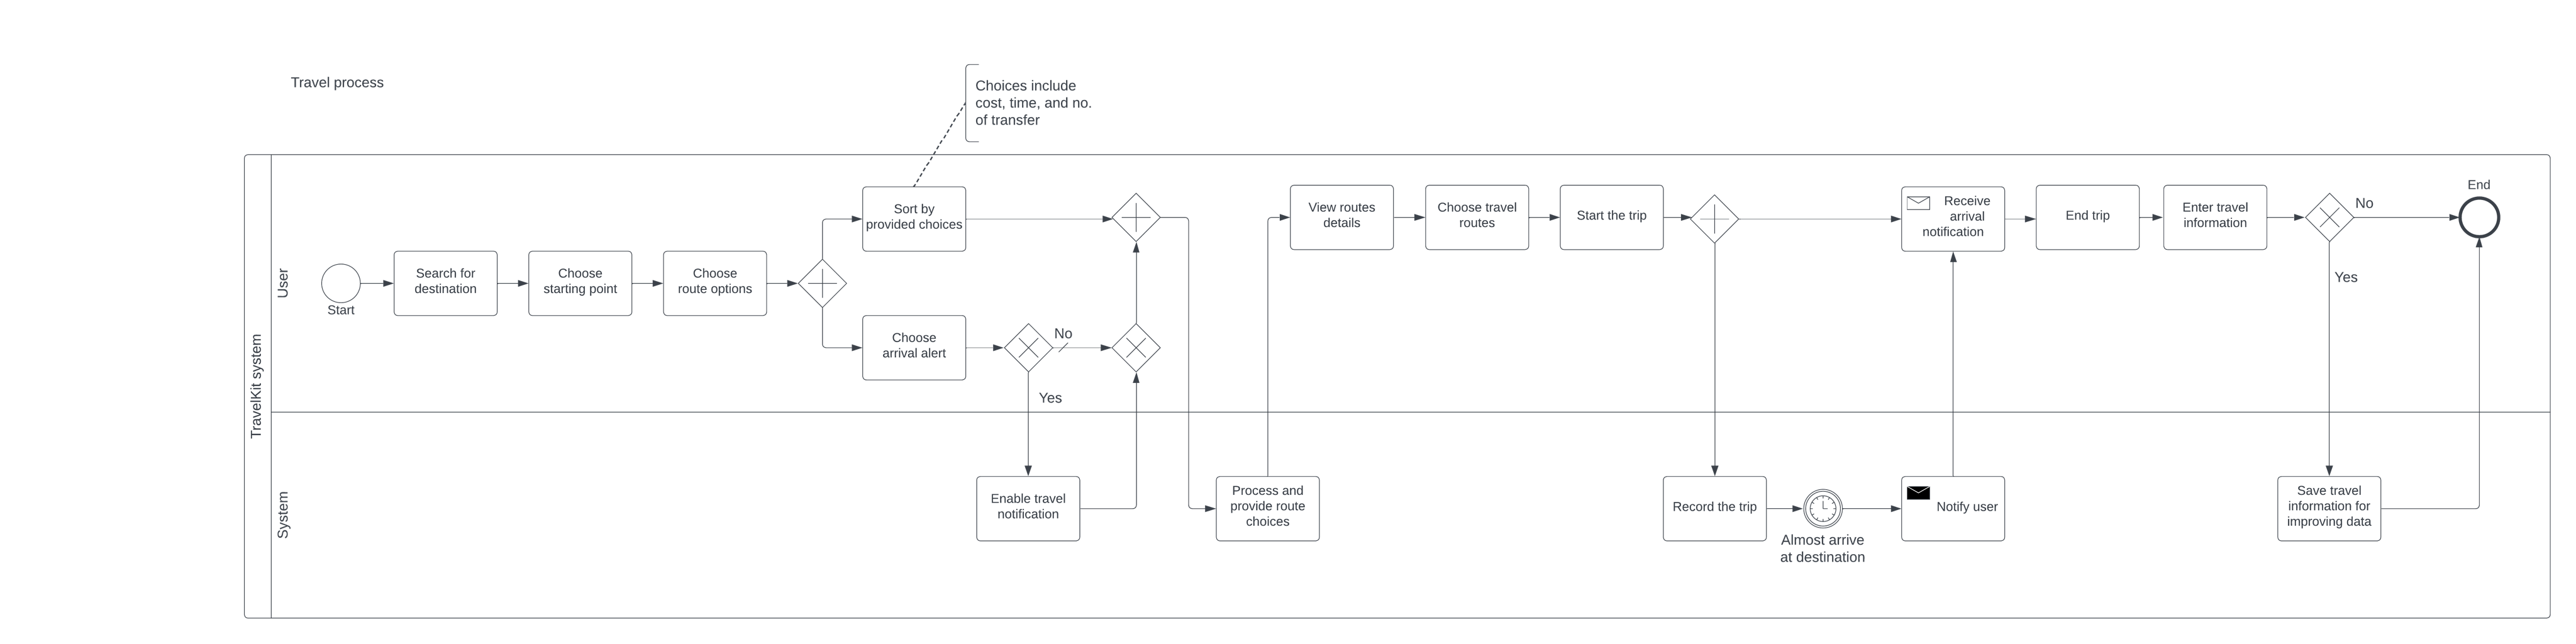
\includegraphics[width=1\linewidth]{chapter3/travel-process.png}
    \caption{Travel process}
    \label{fig:Travel process}
\end{figure}
\par
The travel process for the TravelKit system starts when the user searches for the designated destination. Then, the user will be presented with the default starting point, which the user can either use their current location or select it again. After that, the user will choose their route options, which include the travel cost, time, number of transfers, and the arrival alert. If the user desires to have an arrival alert, the system will enable travel notification. Subsequently, the user can see the provided routes details, choose the route and then start the trip. Meanwhile, the system will start recording the trip and send the notification to the user when they are almost arriving at the destination. Finally, the user can choose either to share their travel route or not. If they choose to do so, the system will save the travel information to improve our system data and user can share to other people in community.

\newpage
\subsection{Community process}
\begin{figure}[!h]
    \centering
    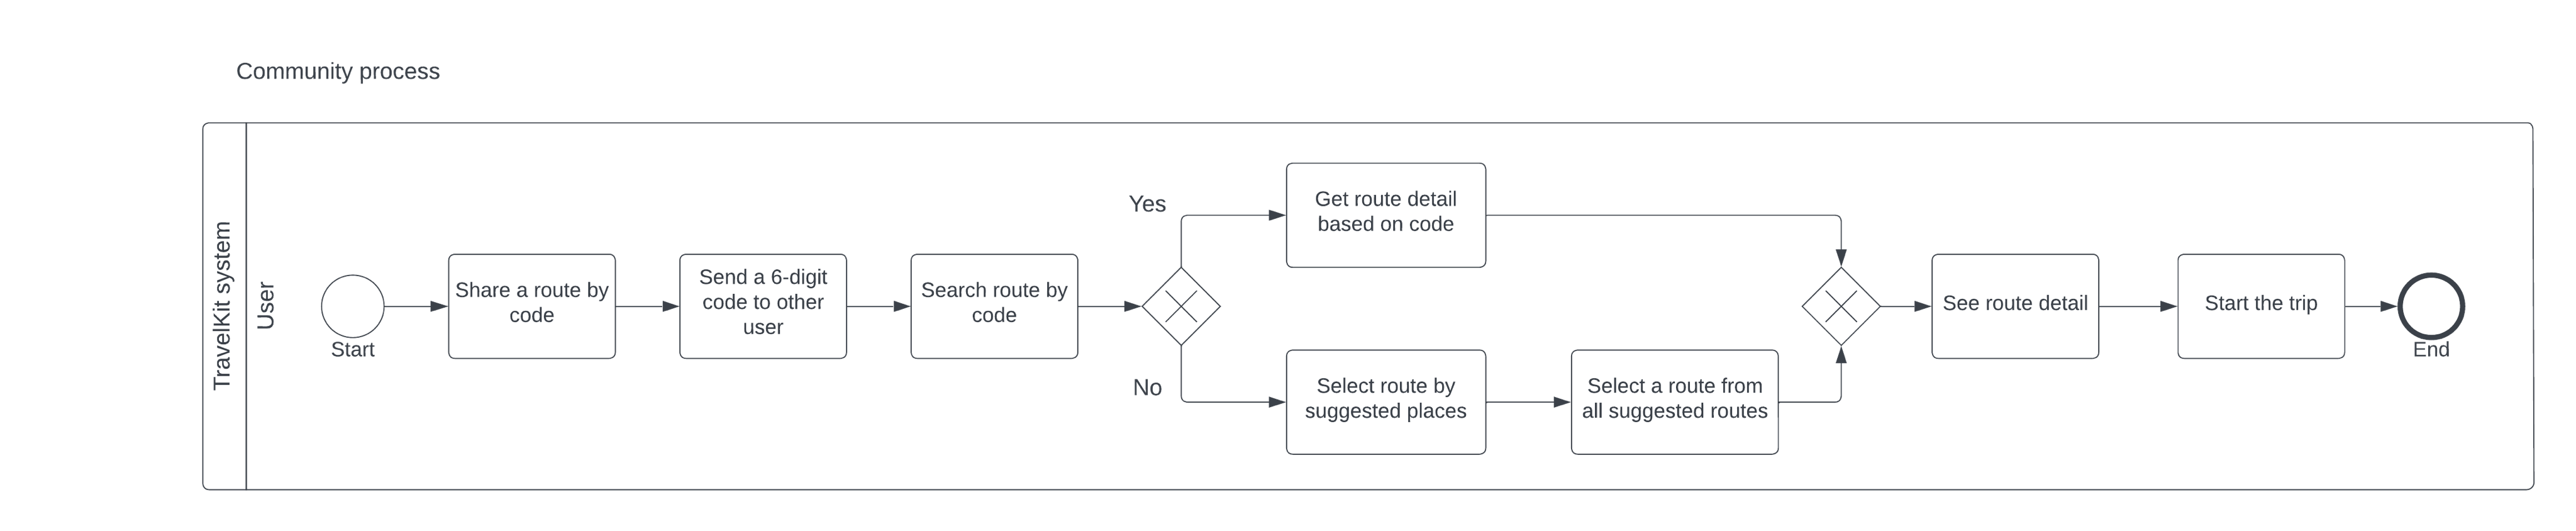
\includegraphics[width=1\linewidth]{chapter3/community-process.png}
    \caption{Community process}
    \label{fig:Community process}
\end{figure}
\par
The community processes for the TravelKit system can be divided into two sub-processes. The first process is for the users who desire to search for routes, which can enter the code to get exact route detail. The second process is for users who wish to find for routes or  places recommendations. The process starts when the user select the destination. Afterwards, the user can view the recommended routes and then select the route they preferred.

\newpage
\section{Database design}
\subsection{Relational Database}
\begin{figure}[!h]
	\centering
	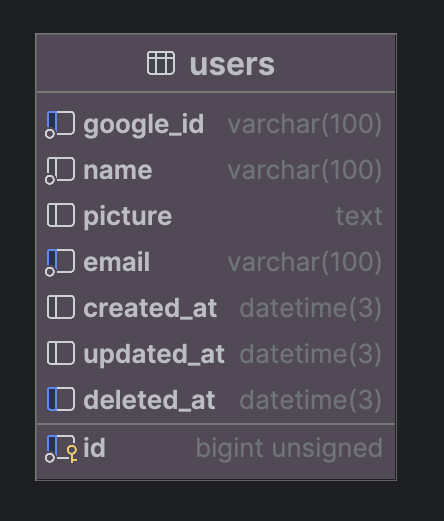
\includegraphics[width=0.5\linewidth]{chapter3/sql-db-schema.png}
	\caption{Relational Database Schema}
	\label{fig:Relational Database Schema}
\end{figure}
Our database relies on MySQL to store user data efficiently. It is intricately connected with MongoDB, particularly in managing community-related information. This dual-database approach enhances functionality, ensuring seamless integration between individual user data and community features, contributing to a robust and scalable system.

\newpage
\subsection{non-relational database}
\begin{figure}[!h]
    \centering
    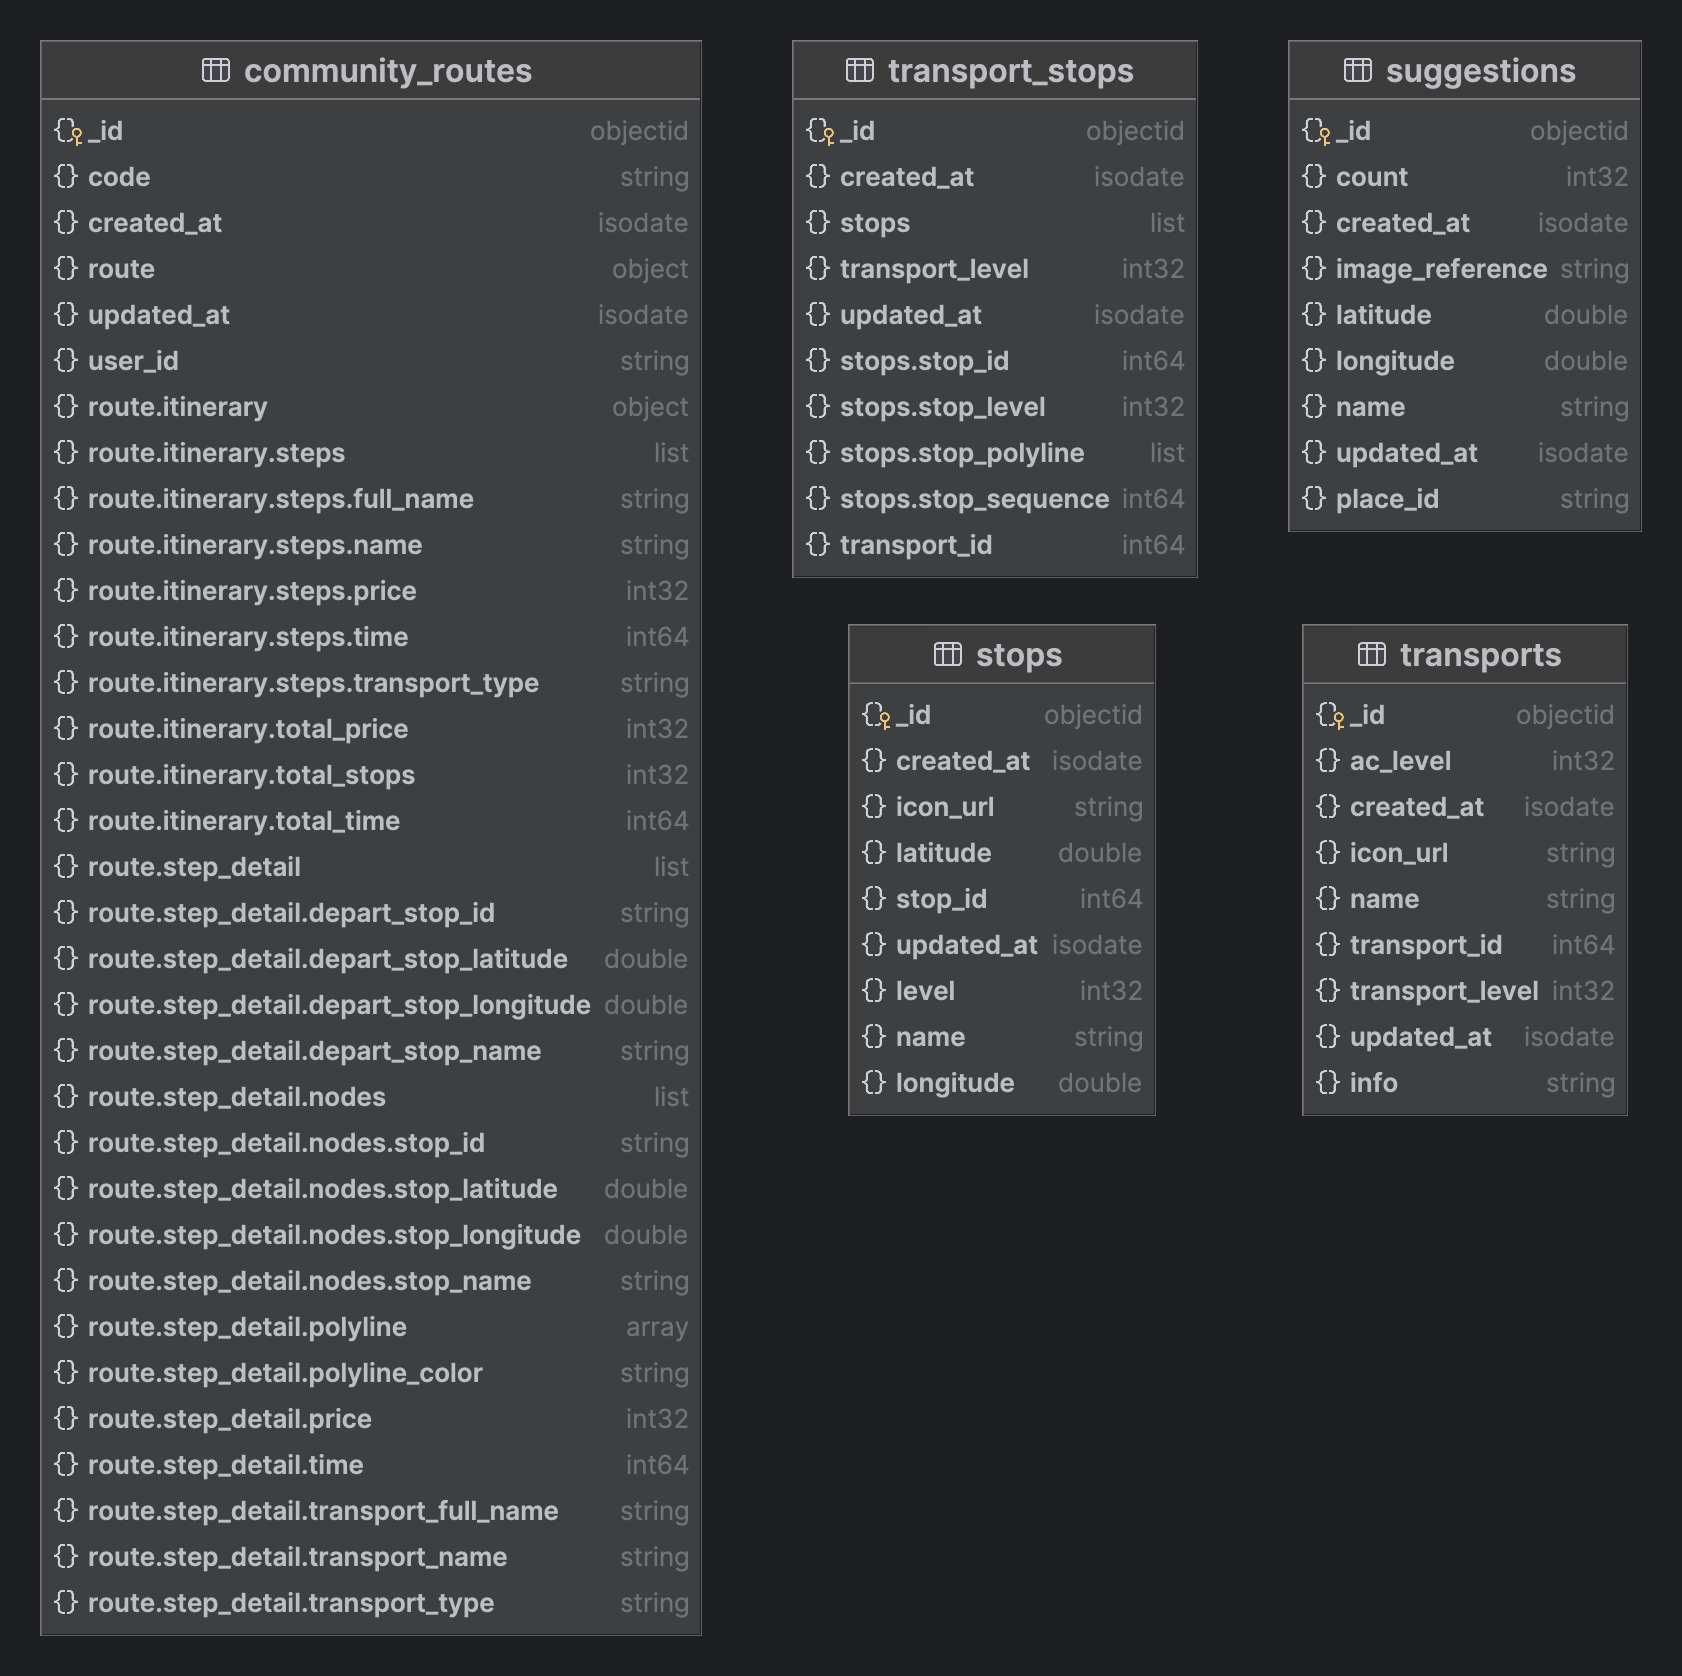
\includegraphics[width=0.6\linewidth]{chapter3/nosql-db-schema.png}
    \caption{Non-Relational Database Schema}
    \label{fig:Non-Relational Database Schema}
\end{figure}
MongoDB is used for storing transport data, stops, and each stop related to each route. It includes:
\begin{itemize}
	\item \textbf{Transports} for storing all data about transport types and transports
	\item \textbf{Stops} for storing stop data, such as bus stops, train stations, and ports
	\item \textbf{Transport Stops} for storing all stops that relate to each transport sequentially
	\item \textbf{Community Routes} for storing shared routes from each users
	\item \textbf{Suggestion} for storing the most frequently selected destinations by users
\end{itemize}

\newpage
\subsection{Graph Database}
The graph database used for storing routes and stops relationship for using the algorithm to find shortest path based on user queries. The graph consist of nodes and relations which is the following node types:
\begin{itemize}
	\item \textbf{STOP} For storing stop or station of all transportation type (e.g. National Theatre, Sanam Luang Bus Terminal, Hua Lamphong, Opposite Tha Phra Chan)
	\item \textbf{ARL} For each line of Airport Rail Link system
	\item \textbf{BRT} For each line of Bus Rapid Transit system
	\item \textbf{BTS} For each line of BTS Skytrain system
	\item \textbf{BUS} For each route of BMTA bus line
	\item \textbf{CHE} For each route of Chao Phraya Express Boat
	\item \textbf{KPS} For each route of minibus and local mini truck
	\item \textbf{MRT} For each line of Metropolitan Rapid Transit
	\item \textbf{SRT} For each line of train
\end{itemize}
\par
Concerning relationships, the project incorporates various types tailored for tasks such as shortest path finding  \cite{neo4j2}, performance optimization, and conditional querying. These relationships are categorized as follows:

\newpage
\subsubsection{GOTO relationship}
\begin{figure}[!h]
	\centering
	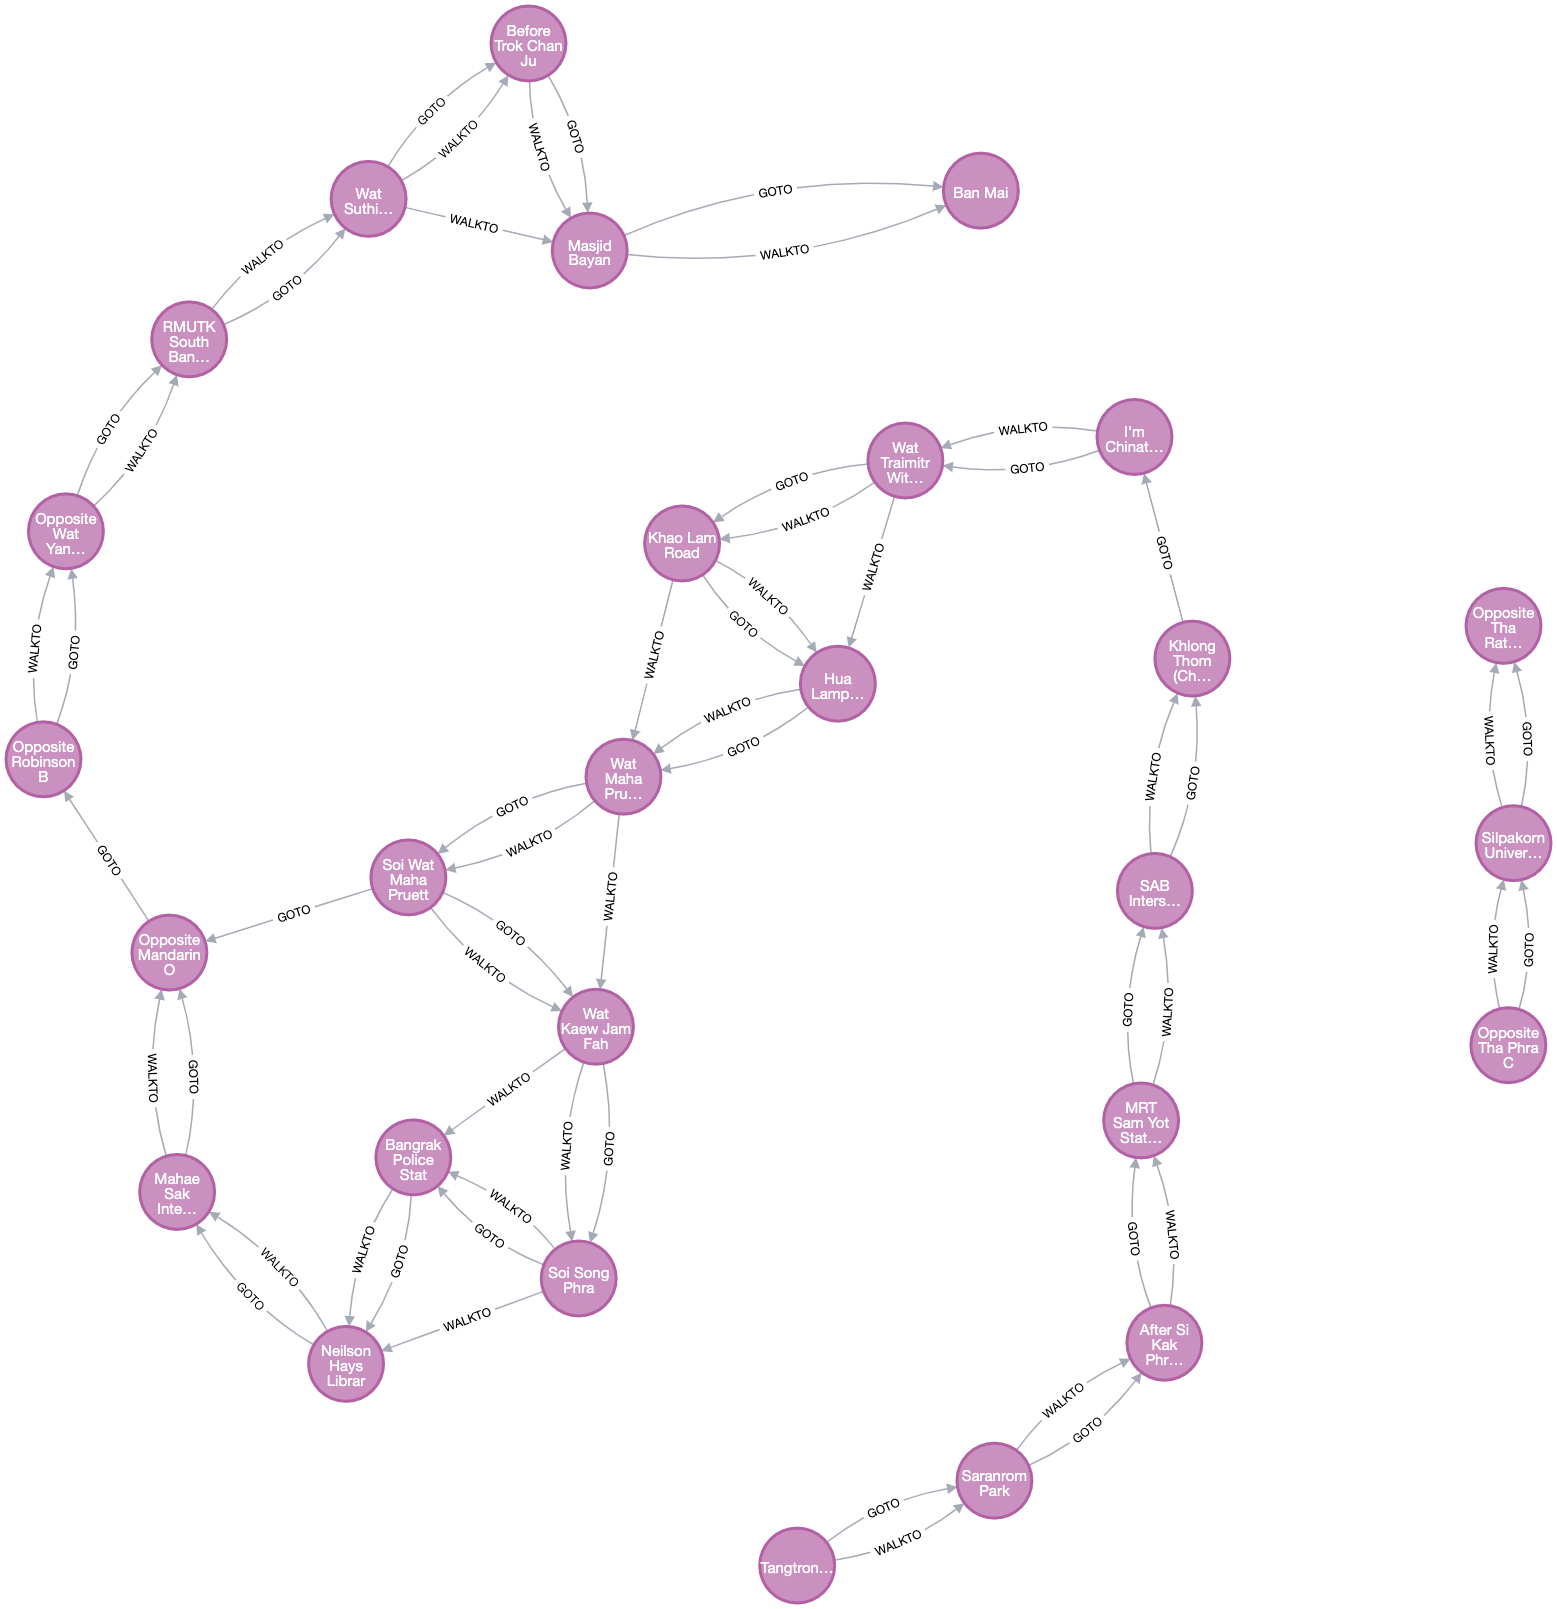
\includegraphics[width=1\linewidth]{chapter3/goto_relationship.png}
	\caption{GOTO relationship}
	\label{fig:GOTO relationship}
\end{figure}
The relation of each two stops that are next to each other and have at least one transportation that pass from one to another (for example, from Sanam Luang stop to National Theatre stop) consider as one-way direction of each side of the road. This relation used for specifying the stop that are available for each bus line to transfer to another

\newpage
\subsubsection{WALKTO relationship}
\begin{figure}[!h]
	\centering
	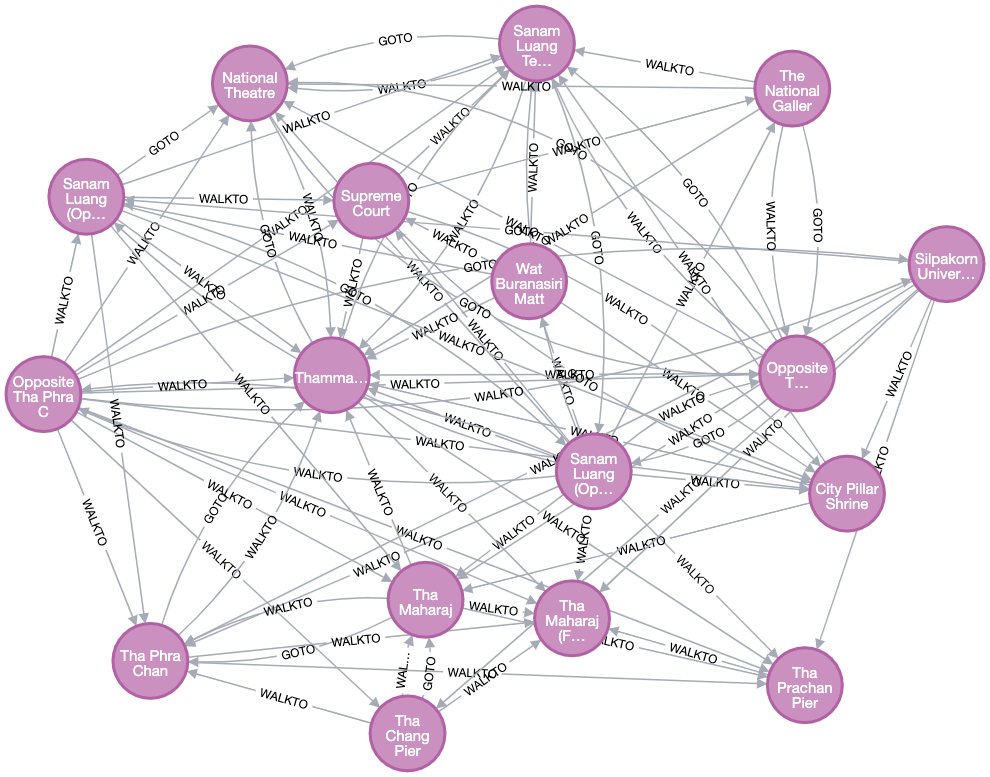
\includegraphics[width=1\linewidth]{chapter3/walkto_relationship.png}
	\caption{WALKTO relationship}
	\label{fig:WALKTO relationship}
\end{figure}
As GOTO relation might not enough for finding the best suitable route, since some stops may not next to each other but user can transfer, walk or reroute between bus line that are in opposite direction for shorter distance. So we create WALKTO relation for all pair of stops that are walkable within 500 meters for querying the route which user can transfer to the nearby stop which are not directly next to each other.

\newpage
\subsubsection{STOPAT/STOPBY relationship}
\begin{figure}[!h]
	\centering
	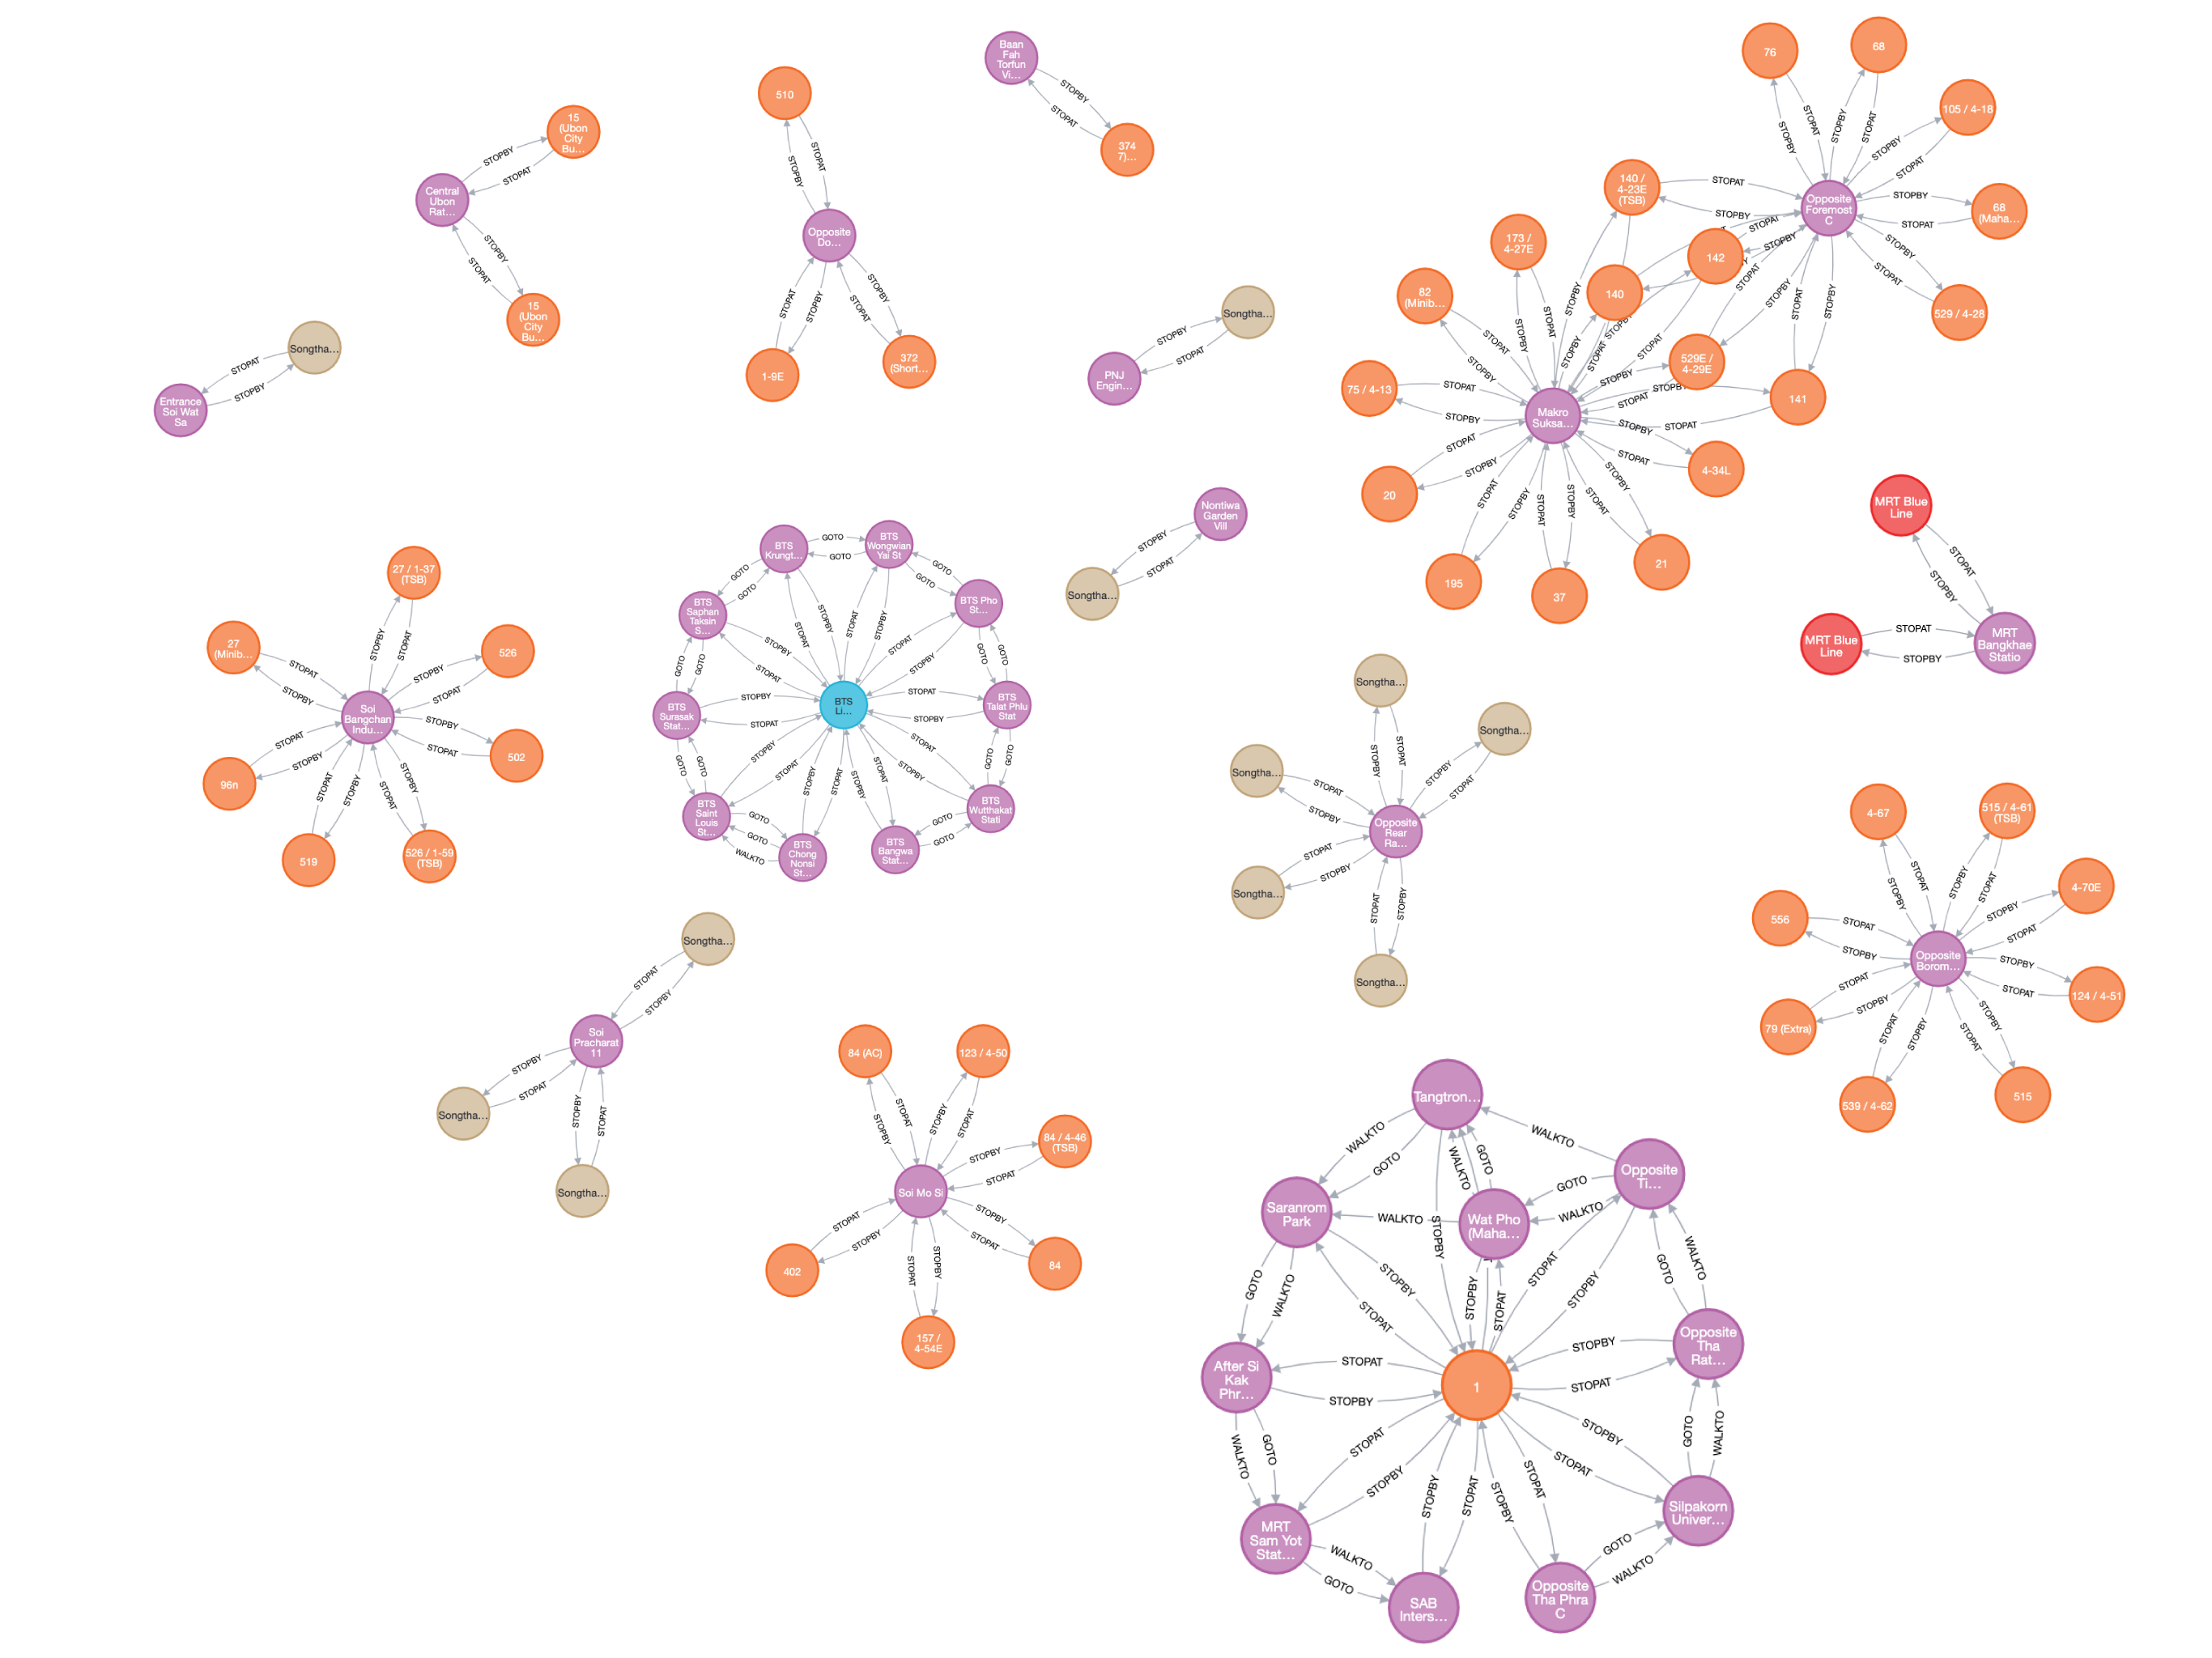
\includegraphics[width=1\linewidth]{chapter3/stopat_relationship.png}
	\caption{STOPAT/STOPBY relationship}
	\label{fig:STOPAT/STOPBY relationship}
\end{figure}
The relationship represent that each transportation line (e.g., bus line, BTS line) are stop at each stop/stations. Each stop are stoppable from many transportation line and each transportation line can pass trough and stoppable at many stop as well.